%!TEX encoding = UTF-8 Unicode
%!TEX root = ../Main/thesis.tex
%!TEX spellcheck = en-US
%%=========================================
\documentclass[../Main/thesis.tex]{subfiles}
\begin{document}
\chapter{Research methodology}
\label{ch:research_methodology}
This chapter describes the research methodology, methods, and frameworks used in this research that addresses the two questions established in Chapter~\ref{ch:reserch_questions}:

\begin{enumerate}
	\item \textbf{How can BLE beacons be used to support firefighter movement tracking under smoke diving training?}
	\item \textbf{Do the beacons provide good enough information for useful feedback?}
\end{enumerate}

\section{Design Science}
Design Science is a research methodology that establishes and uses research when the goal is an artifact or a recommendation.
Research based on design science can be performed in an organizational context or an academic environment \citep{lacerda2015design}.
As the goal of this research is to create and evaluate an artifact, the design science methodology fits well.

\citet{hevner2004design} claims that design is both a process and an artifact.
The design process produces an innovative artifact, which is evaluated to provide feedback about the artifact itself, and a better understanding of the problem. 
This information is used to improve both the artifact itself and the design process.

Design Science can be seen as a problem solving process.
The foundation on which design science is based is that knowledge about, and understanding, of a design problem, and the solution to that problem, is something you achieve through the development and use of an artifact.
Artifacts as a result of design science is according to \citet{March1995} \textit{constructs}, \textit{models}, \textit{methods}, and \textit{instantiations}.

%\todo{Add more about how and why I use design science}

\subsection{Artifacts}
Within design science artifacts are created to address unsolved problems, and when they are evaluated by looking at the utility they provide in solving the problem.
\citet[p.78-79]{hevner2004design} identify those four artifacts as follows:

\begin{enumerate}
	\item \textit{Constructs}: provides the language, vocabulary and concepts, which are used to define and communicate the problems and solutions.
	\item \textit{Models}: are representations of a real world situation of the design problem and its solution space created using constructs. They help with the understanding of the problem and the solution, and is often used to represent the connection between them. 
	\item \textit{Methods}: provide guidance on how to search the solution space and solve problems.
	\item \textit{Instantiations}: is an implementation of a construct, model or method in a working system.
\end{enumerate}

In this research the main artifact is the back end of the FireTracker system, which determines the movements and activity of the fire fighters based on the collected data, thus, it is an instantiation.

\subsection{Guidelines}
\citet{hevner2004design} defines a set of seven guidelines for implementing and evaluating design science research.
Those guidelines and their definitions are listed in table~\ref{tab:design-science-guidelines}.
The guidelines gives the researchers clear requirements for executing design science research.
Using these guidelines and focusing on quality, efficiency, and functionality makes it easier to satisfy the requirements of design science research. 
The guidelines will be used throughout the process of this research to ensure that it is conducted properly.

\begin{table}[h]
\centering
\caption[Design Science Research Guidelines]{Design Science Research Guidelines \citep[p.83]{hevner2004design}}
\begin{tabular}{|p{0.4\linewidth}|p{0.55\linewidth}|}
	\hline
	\textbf{Guideline} & \textbf{Description} \\ \hline
	Guideline 1: Design as an Artifact & Design-science research must produce a viable artifact in the form of a construct, a model, a method, or an instantiation. \\ \hline
	Guideline 2: Problem relevance & The objective of design-science research is to develop technology-based solutions to important and relevant business problems. \\ \hline
	Guideline 3: Design evaluation & The utility, quality, and efficacy of a design artifact must be rigorously demonstrated via well-executed evaluation methods. \\ \hline
	Guideline 4: Research contributions & Effective design-science research must provide clear and verifiable contributions in the areas of the design artifact, design foundations, and/or design methodologies. \\ \hline
	Guideline 5: Research rigor & Design-science research relies upon the application of rigorous methods in both the construction and evaluation of the design artifact. \\ \hline
	Guideline 6: Design as a search process & The search for an effective artifact requires utilizing available means to reach desired ends while satisfying laws in the problem environment. \\ \hline
	Guideline 7: Communication of research & Design-science research must be presented effectively both to technology-oriented as well as management-oriented audiences. \\ \hline
\end{tabular}
\label{tab:design-science-guidelines}
\end{table}

\section{Interaction Design Lifecycle}
Figure~\ref{fig:method-diagram} illustrates the development process used in this research
This development process is a variation of the interaction design lifecycle.
The first iteration of the project is establishing requirements and creating design alternatives.
This iteration is described in Chapter~\ref{ch:requirements}.
Then there are two iterations of developing prototypes, evaluating them and creating new requirements.
These iterations are described in Chapter~\ref{ch:development-1}~and~\ref{ch:development-2}.
The last iteration is the final evaluation of the product, which is described in Chapter~\ref{ch:evaluation}.
\newpage

\begin{figure}[h]
	\centering
	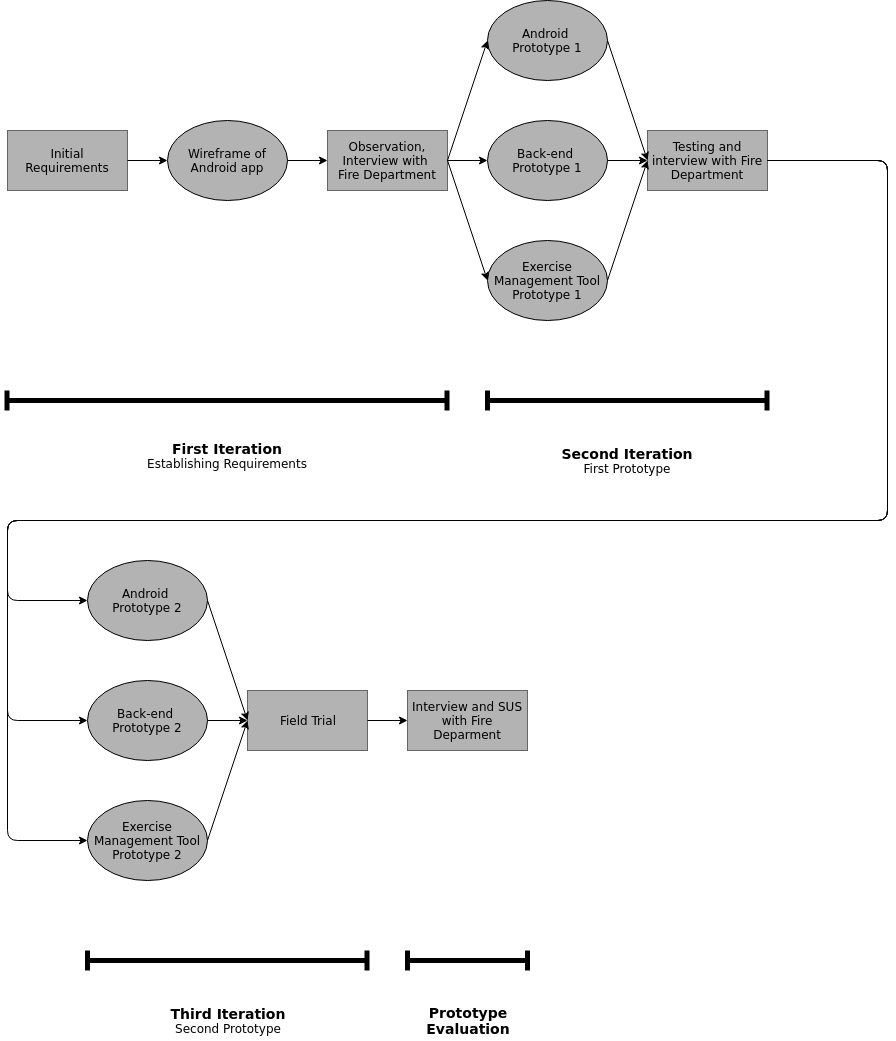
\includegraphics[width=\textwidth]{../fig/Method-diagram}
	\caption{Overview of the development process}
	\label{fig:method-diagram}
\end{figure}

\citet{Preece2011} defines a lifecycle model for interaction design.
This model is a simplified version of reality, and it is intended as an abstraction.
An overview of this model is shown in Figure~\ref{fig:interaction-design-lifecycle}.

\begin{figure}[h]
	\centering
	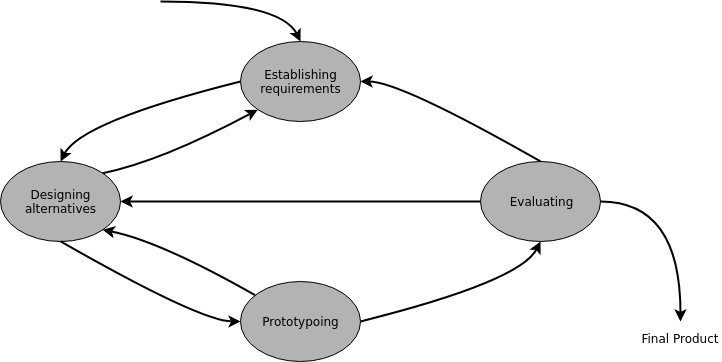
\includegraphics[width=\textwidth]{../fig/Interaction-design-lifecycle}
	\caption[A simple interaction design lifecycle model]{A simple interaction design lifecycle model \citep[p.332]{Preece2011}}
	\label{fig:interaction-design-lifecycle}
\end{figure}


In their model \citet{Preece2011} divides the interaction design process into four basic activities: \textit{Establishing Requirements}, \textit{Designing Alternatives}, \textit{Prototyping}, and \textit{Evaluating}.
These are briefly described below.

\subsection{Establishing Requirements}
To create something that can support people, one needs to know who those people are, and what kind of support a product can provide. 
This need for support forms the requirements for the product.
Establishing requirements is very important in interaction design, and a fundamental part of a user-centered approach to development \citep{Preece2011}.

\subsection{Designing Alternatives}
Designing alternatives is the core activity of the interaction design lifecycle: suggesting ideas for meeting the requirements.
It can be divided into two sub-activities: conceptual design and concrete design.
Conceptual design is creating an abstraction or model of the product, and how it can be used.
Concrete design is determining details of the actual product, involving choosing colors, sounds, and images \citep{Preece2011}.

\subsection{Prototyping}
Prototyping is the creation of a prototype using one or more of the techniques described in Section~\ref{sec:prototyping}.

\subsection{Evaluating}
Evaluation is determining the usability and acceptability of the product measured in terms of usability and user experience criteria.
In interaction design a high level of user involvement is required throughout the development process to enhance the chance of delivering an acceptable product \citep{Preece2011}.

\section{Prototyping}
\label{sec:prototyping}
A prototype is a early version of a product. 
It is supposed to demonstrate some features or properties of an artifact which can be evaluated and analyzed to gain some understanding about how the product can be revised in the next iteration of the development \citep{oates2005researching}.
There are two types of prototypes: \textit{low-fidelity-prototype} and \textit{high-fidelity-prototype}
The goal of prototyping is to get user feedback.

Low-fidelity prototyping is a way of translating high-level designs into testable artifacts \citep{Babich2017}.
The purpose of a low-fidelity prototype is to test and check functionality, not visual designs and appearances.
In a low-fidelity prototype only the most important elements of the content is included, and only general visual attributes are presented.

High-fidelity prototypes look and function as similar to the actual product as possible \citep{Babich2017}.
They are usually created when there is a solid understanding of the final product and it needs to be tested on actual users.
In a high-fidelity prototype most of the content is included, and the design is realistic with all details in place.

In this research the goal is to create a High-fidelity prototype with tracking-functionality. 

\section{Data Collection}
Collecting data is an important part of the research process, and therefore choosing the right methods also important.
This section presents the methods used in this project: observation, semi-structured interview, field-trial, technical testing, and questionnaire.

\subsection{Observation}
Observation is a data gathering technique that can be used at any stage in the development process.
During observation the user can be observed directly by the investigator, or indirectly through video or audio recordings.
There are two main types of observation: controlled environment observation and field environment observation \citep{Preece2011}.

Observations will be used to set the initial requirements, and during testing and evaluation.

\subsubsection{Controlled Environment}
Observation in a controlled environment often happen in a laboratory-like where the observer has the possibility to control different factors that can influence the testing.
Controlled environment observations are more formal in their character than field environment observations \citep{Preece2011}.
The observations in the technical testing in iteration 3 will be made in controlled environment.

\subsubsection{Field Environment}
Observation in a field environment is used when observing a user in their natural environment.
They are useful as it can be difficult for users to explain what they do, and how they think, when solving a task \citep{Preece2011}.
A field environment was used in the field trial of the final prototype.

\subsection{Interview}
Interviews are one of the most common techniques for collecting qualitative data.
There are three types of qualitative interviews: unstructured interview, semi-structured interview, and individual in-depth interview \citep{DiCicco-Bloom2006}.
The interviews in this project was conducted as semi-structured interviews.

A semi-structured interview combines the features of unstructured and structured interviews and use both open and closed questions \citep{Preece2011}.
The general way of performing a semi-structured interview is to have a set of open questions which is used as guidance, and with open answers to inquire as much information as possible.
From those open questions other new questions can emerge during the interview \citep{DiCicco-Bloom2006}.

Semi-structured interviews will be used to establish requirements, and to get feedback from the firefighters during the development process and in the evaluation. 

\subsection{Technical Testing}
Technical testing will be done as experiments in this research.
Experiments are scientific procedures with the purpose of either testing a hypothesis, making a discovery, or demonstrating a known fact.
The core part of an experiment is to collect data under specific and controlled circumstances \citep{Hellevik2002}.

Technical testing will be used to improve the prototypes in iteration 3.

\subsection{Field Trial}
Field trials, or field experiments, are experiments where the researchers observe events in a real-life setting instead of in a laboratory setting \citep{oates2005researching}.
In field trials the researcher cannot control all variables in the same way as in a laboratory experiment.

Field trials will be used to test the final prototype.

\subsection{System Usability Scale Questionnaire}
\begin{figure}[h]
	\centering
	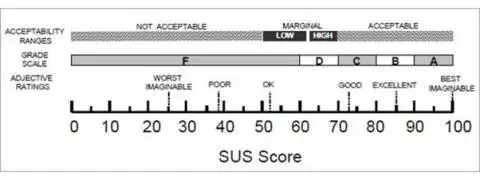
\includegraphics[width=\textwidth]{../fig/sus-score}
	\caption[SUS scores and how they can be interpreted]{SUS scores and how they can be interpreted \citep{Brooke2013}.}
	\label{fig:sus-score}
\end{figure}

The System Usability Scale (SUS) is a scale used to quickly measure how people perceive the usability of a system they are working with \citep{Brooke2013}.
It is a questionnaire with ten questions, five of them positively worded, and five negatively worded.
This is done to avoid response biases \citep{Brooke2013}.

The respondent answer each question on a five point scale from Strongly agree to Strongly disagree \citep{AssistantSecretaryforPublicAffairs2013}.
The overall SUS score for the system is then calculated on a scale from 1 to 100, where a score between 68 and 100 is considered an acceptable or good usability score, as shown in Figure~\ref{fig:sus-score} \citep{AssistantSecretaryforPublicAffairs2013}.

The System Usability Scale will be used to get feedback on the firefighter's perception on the final prototype.


\section{Summary}
This chapter has described the research methodology and methods that will be used in this research. 

\blankpage


\onlyinsubfile{\bibliographystyle{chicago}}
\onlyinsubfile{\bibliography{../library}}
\end{document}
